\section{AI动画}

在动画领域,人工智能(AI)正以其强大的技术力量掀起一场前所未有的变革。AI动画的出现,不仅是技术的进步,更是艺术创作的一次深刻革命。它利用先进的算法和模型,从角色设计到场景渲染,从动作捕捉到特效生成,全方位重塑了动画制作的流程。

以近期备受瞩目的国产动漫电影《哪吒2》为例,AI技术贯穿了从前期设计到后期制作的全流程。AI辅助设计系统能够快速生成角色概念图,大大缩短了创作周期;AI动作捕捉技术精准记录演员表演,并将其转化为数字角色的动作数据;AI渲染引擎则通过深度学习算法,实现了更加真实的光影效果和材质表现。这种技术的应用不仅提升了制作效率,更突破了传统动画制作的局限,为观众带来了前所未有的视觉体验。

在角色设计方面,AI通过学习大量数据,能够生成符合特定主题或风格的独特角色设计,并实现风格迁移和个性化定制。而在动画制作过程中,AI技术可以自动生成动作和表情,减少人工绘制的工作量,同时利用动态捕捉技术实现更逼真的表现。此外,AI还能自动生成动画中的特效,如烟雾、火焰、水波等,进一步提升视觉效果。

AI动画的崛起,不仅改变了动画的制作方式,更拓展了其应用场景。从教育类动画到广告动画,AI能够根据不同的需求进行个性化定制,满足不同观众群体的偏好。这种高度的灵活性和适应性,使得AI在动画领域的应用前景愈发广阔。

然而,AI动画的发展也带来了新的挑战。一方面,确保生成动画的高质量并非易事;另一方面,传统动画技能可能面临被掩盖的风险。尽管如此,AI与传统动画方法的结合,仍为动画师和内容创作者提供了无限的可能性。随着技术的不断进步,AI动画的未来充满希望,它将继续推动动画产业迈向新的高度。

下面以郑和下西洋为背景,使用AI工具制作一个简单的动画。

\prompt{生成30秒的郑和下西洋动画剧本,包含船队出发、海上航行、异国贸易三个场景}


\begin{gptbox}
\small{
  \textbf{《郑和下西洋》动画剧本}

  \textbf{场景一:船队出发}
  \begin{itemize}
      \item \textbf{镜头1:南京城外港口}
      \begin{itemize}
          \item \textbf{画面}:清晨,南京城外港口,宝船队整齐排列,旗帜飘扬,人群欢呼。
          \item \textbf{旁白}:公元1405年,郑和奉命下西洋,船队从南京出发,开启伟大征程。
          \item \textbf{音乐}:激昂的古风音乐,带有海浪声。
      \end{itemize}
  \end{itemize}
  
  \textbf{场景二:海上航行}
  \begin{itemize}
      \item \textbf{镜头2:海上航行}
      \begin{itemize}
          \item \textbf{画面}:船队在波涛中前行,海浪翻腾,船员们忙碌操作。
          \item \textbf{旁白}:船队穿越惊涛骇浪,凭借罗盘和星图,勇往直前。
          \item \textbf{音乐}:紧张的鼓点声,模拟航行的艰难。
      \end{itemize}
  \end{itemize}
  
  \textbf{场景三:异国贸易}
  \begin{itemize}
      \item \textbf{镜头3:异国港口}
      \begin{itemize}
          \item \textbf{画面}:船队抵达异国港口,当地居民热情迎接,贸易市场热闹非凡。
          \item \textbf{旁白}:郑和与各国通商,传播友谊,带回珍宝。
          \item \textbf{音乐}:欢快的异域风情音乐,营造繁荣氛围。
      \end{itemize}
  \end{itemize}

}
\end{gptbox}

% Generate a script for a 30-second animated short film on the theme of “Zheng He's Voyages to the Western Seas,” including the following three scenes:Departure of the Fleet: Depict the grand scene of Zheng He's fleet setting sail from the port outside Nanjing during the Ming Dynasty.Sea Voyage: Show the fleet navigating through the stormy seas, overcoming challenges in a tense sequence.Foreign Trade: Present the fleet arriving at a foreign port and engaging in prosperous trade with the local people in a friendly manner.The script should be concise and highlight the core plot and atmosphere of each scene, suitable for quick storytelling.

接着使用AI视频生成工具Pix Verse\footnote{\url{https://aipixverse.com}},使用上述剧本对应的英文作为提示词得到视频,分别如\reffig{fig:anime-video}所示。

\fig[h]{
    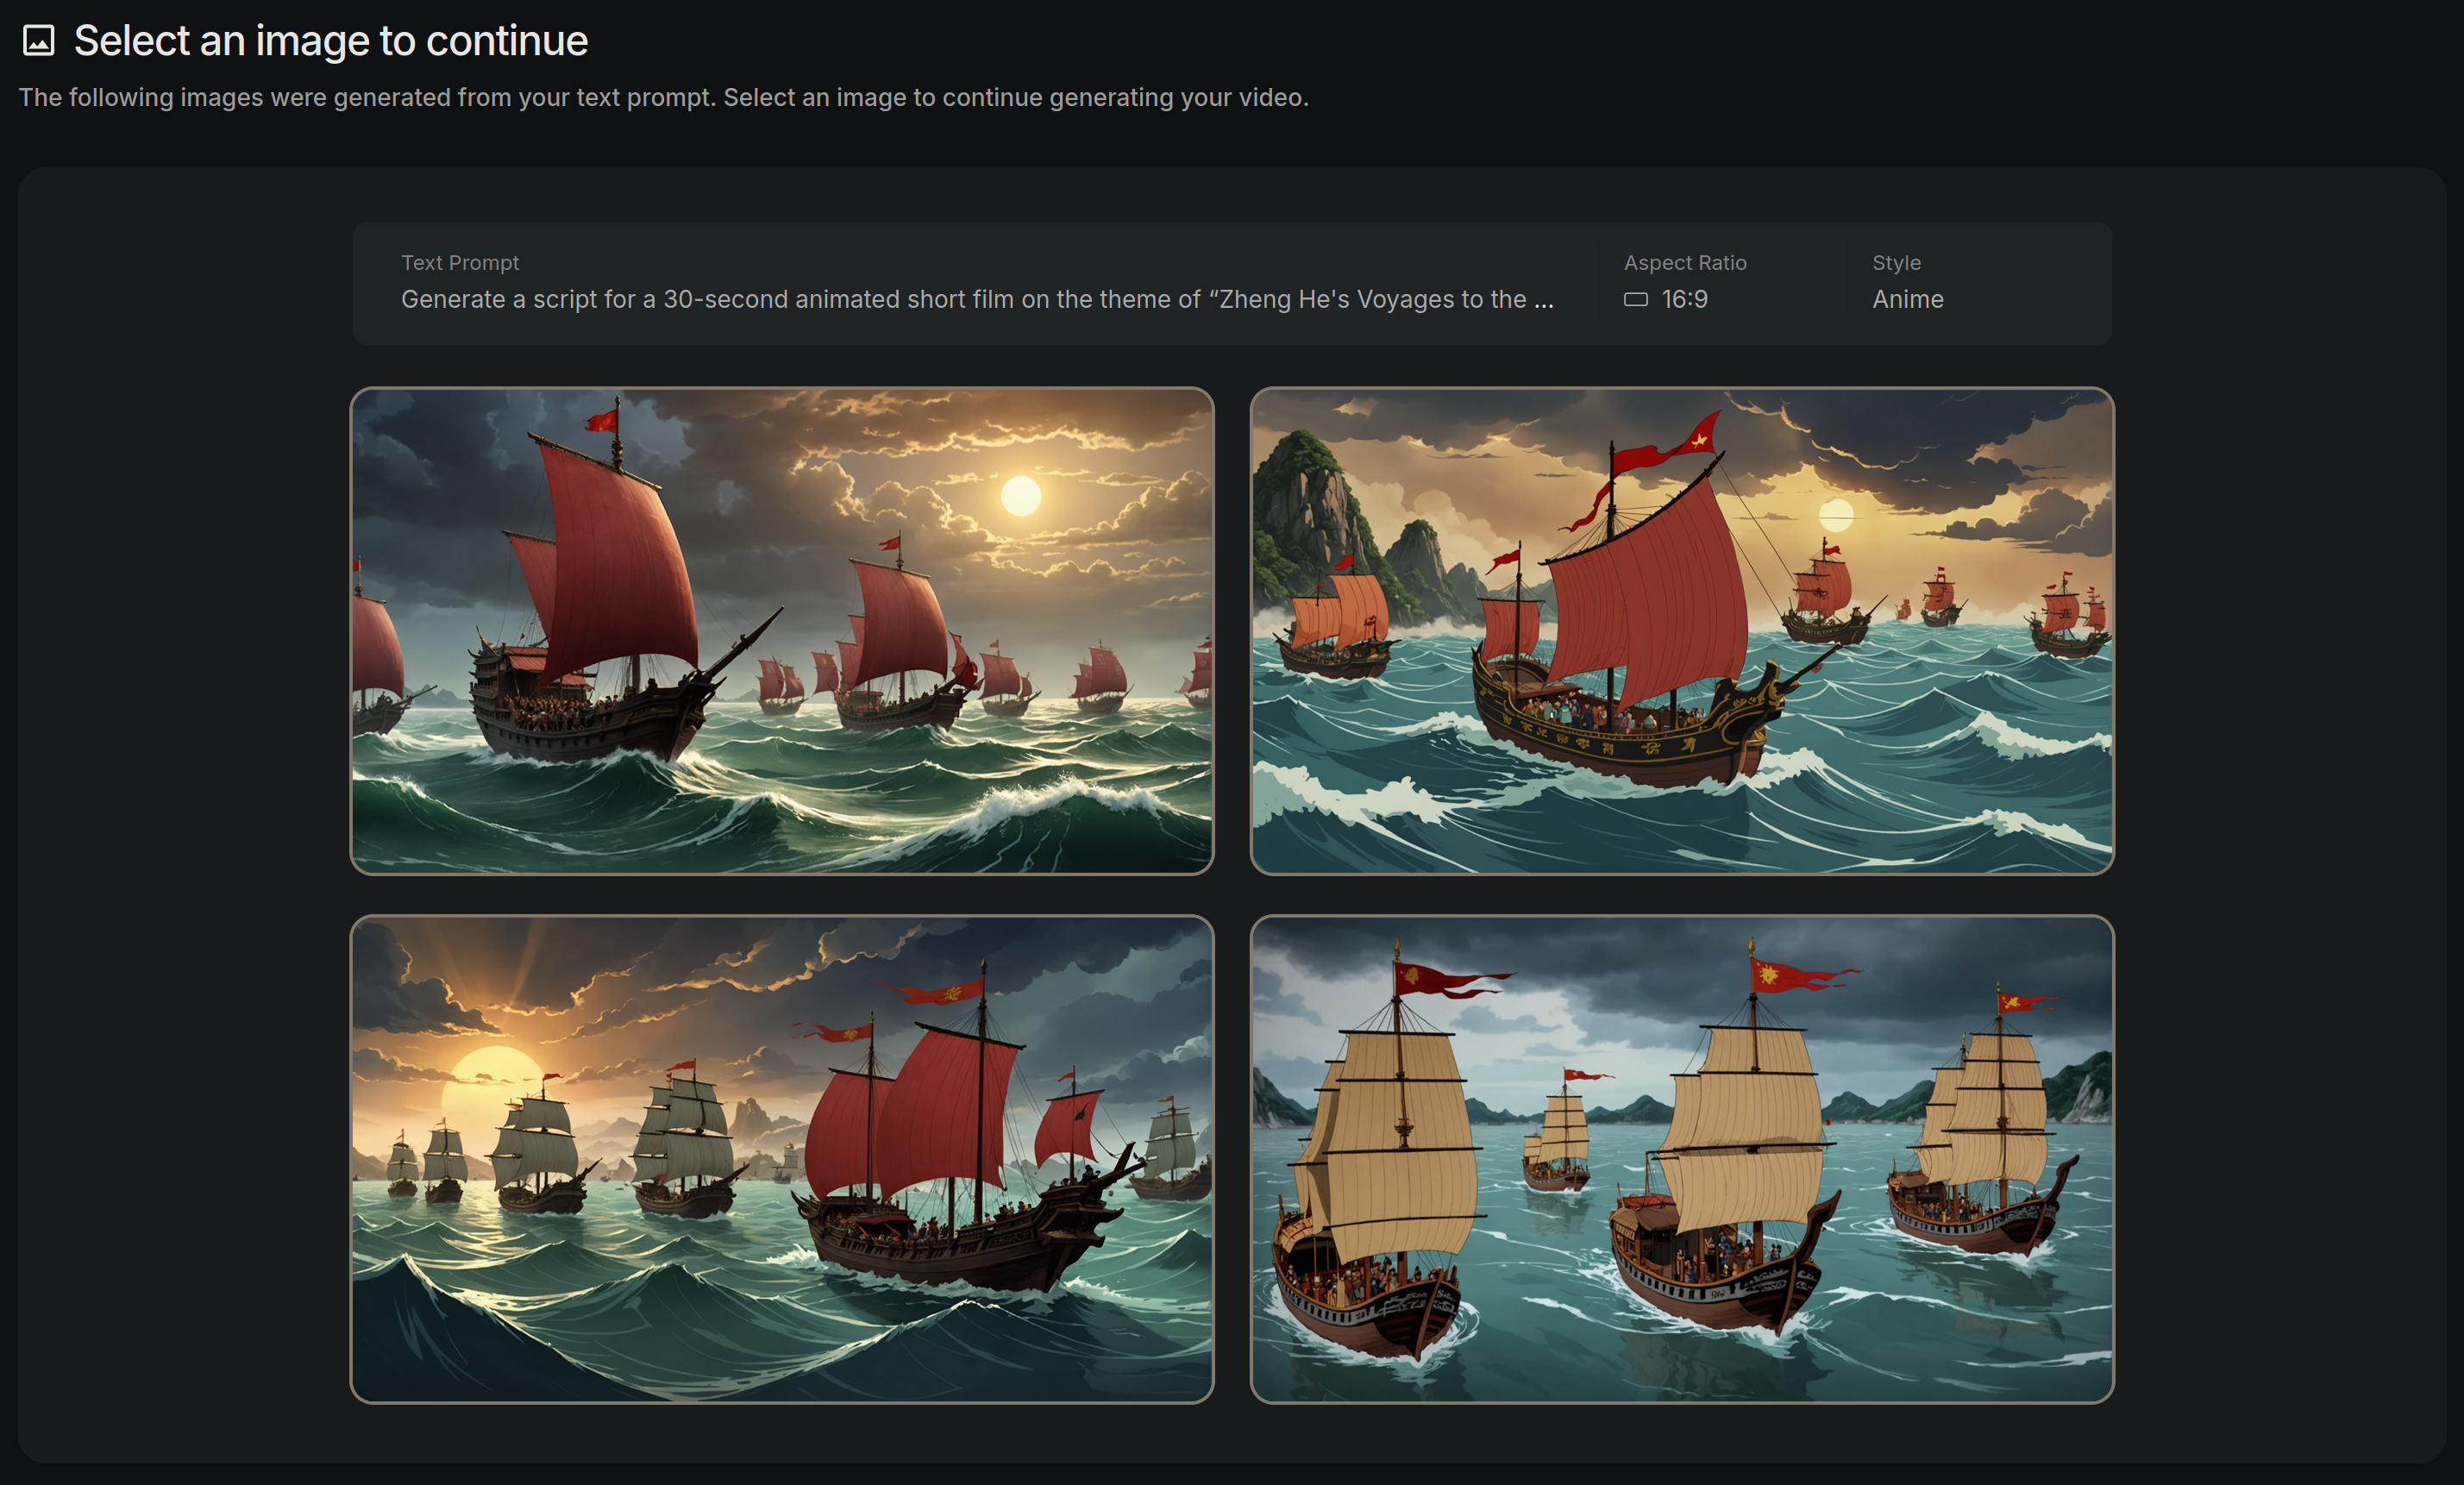
\includegraphics[width=0.7\textwidth]{style-select}
    \caption{视频结果}
    \label{fig:anime-video}
}

% \item
%   \textbf{分镜脚本}
%   Prompt:
%   \prompt{``将上述剧本转为Blender分镜脚本,包含镜头角度、时长、物体运动参数''}

%   GPT输出:
%   \begin{gptbox}
%   \small{
%   \begin{lstlisting}[language=Python]
%     # 场景1镜头设置
%     camera.location = (0, -10, 5)
%     camera.rotation_euler = (radians(60),0,0)
%     ship.animation_keyframes = [
%       (1, (0,0,0)), 
%       (300, (0,15,0)) # 300帧内沿Y轴移动15单位
%     ]
%   \end{lstlisting}
%   }
%   \end{gptbox}
% \item
%   \textbf{自动生成代码} Prompt:
%   \prompt{``写Blender Python脚本创建明代宝船模型,长44丈(按1:100比例)''}

%   GPT输出:

%   \begin{gptbox}
%   \small{
%   \begin{lstlisting}[language=Python]
%     import bpy
%     # 创建船体
%     bpy.ops.mesh.primitive_cylinder_add(radius=2.2, depth=14)
%     hull = bpy.context.object
%     hull.name = "Ming_Ship_Hull"
%     # 添加桅杆
%     bpy.ops.mesh.primitive_cylinder_add(radius=0.3, height=8)
%     mast = bpy.context.object
%     mast.location = (0, 0, 4)
%   \end{lstlisting}
%   }
%   \end{gptbox}
% \end{enumerate}




